
\newif\ifvimbug
\vimbugfalse

\ifvimbug
\begin{document}
\fi

\exercise{Reinforcement Learning}

You recently acquired a robot for cleaning you apartment but you are not happy with its performance and you decide to reprogram it using the latest AI algorithms. As a consequence the robot became self-aware and, whenever you are away, it prefers to play with toys rather than cleaning the apartment. Only the cat has noticed the strange behavior and attacks the robot. The robot is about to start its day and its current perception of the environment is as following 
%
\begin{center}
	%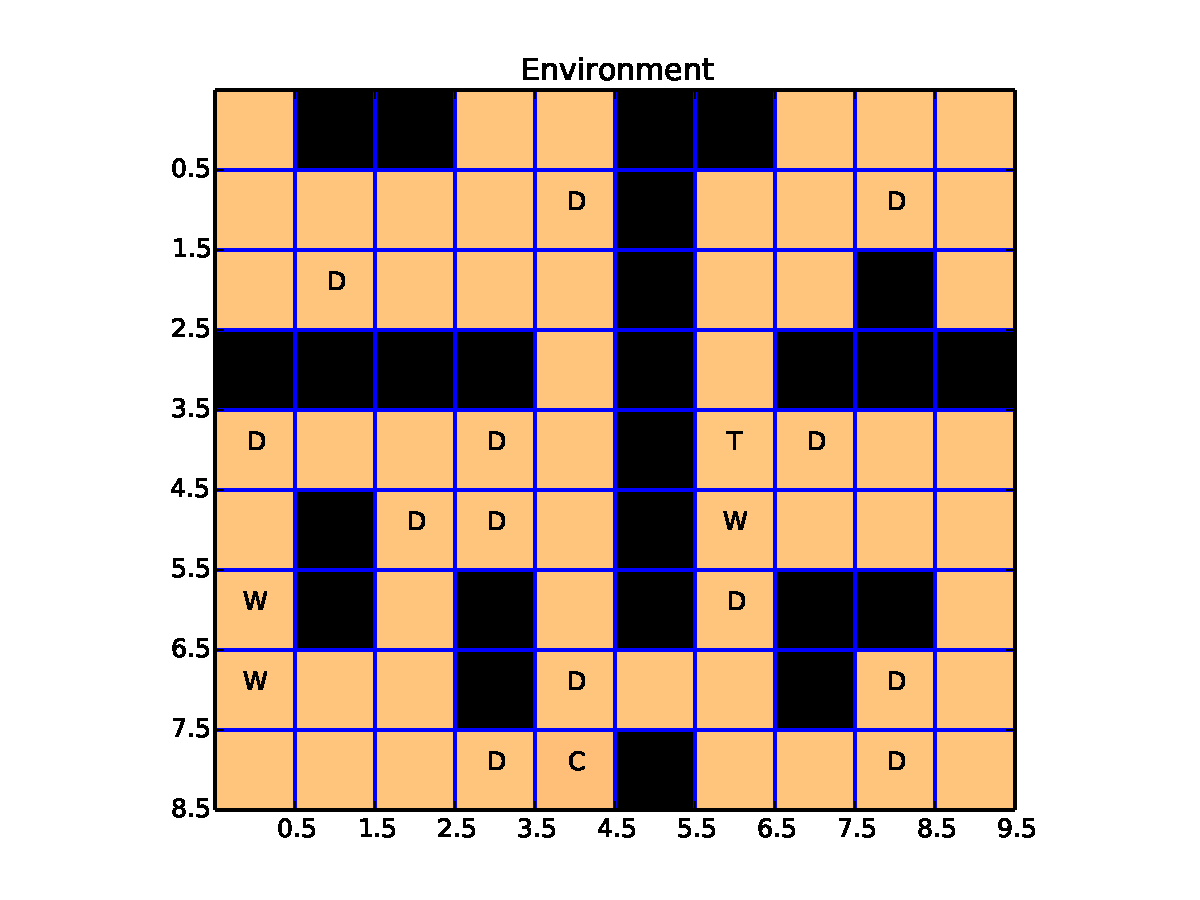
\includegraphics[width=0.75\textwidth]{fig/gridworld.pdf}
	\colorbox{yellow}{Your graphic could be here. It just wasn't included.}
\end{center}
%
The black squares denote extremely dangerous states that the robot must avoid to protect its valuable sensors. The reward of such states is set to $r_\textrm{danger}=-10^5$ (NB: the robot can still go through these states!). Moreover, despite being waterproof, the robot developed a phobia of water (W), imitating the cat. The reward of states with water is $r_\textrm{water}=-100$. The robot is also afraid of the cat (C) and tries to avoid it at any cost. The reward when encountering the cat is $r_\textrm{cat}=-3000$. The state containing the toy (T) has a reward of $r_\textrm{toy}=1000$, as the robot enjoys playing with them. Some of the initial specification still remain, therefore the robot receives $r_\textrm{dirt}=35$ in states with dirt (D).

State rewards can be collected at every time the robot is at that state. 
The robot can perform the following actions: \textit{down, right, up, left} and
\textit{stay}.

In our system we represent the actions with the an ID (0, 1, 2, 3, 4), while the grid is indexed as $\{ \texttt{row}, \texttt{column} \}$. The robot can't leave the grid as it is surrounded with walls.
A skeleton of the gridworld code and some plotting functions are available at the webpage.
For all the following questions, always attach a snippet of your code.


\begin{questions}

\begin{question}{Finite Horizon Problem}{14}
In the first exercise we consider the finite horizon problem, with horizon $T=15$ steps.
The goal of the robot is to maximize the expected return 
\begin{equation}
J_\pi = \mathbb{E}_\pi\left[\sum_{t=1}^{T-1}r_t(s_t,a_t)+r_T(s_T)\right], \label{Eq:J}
\end{equation}
according to policy $\pi$, state $s$, action $a$, reward $r$, and horizon $T$. Since rewards in our case are independent of the action and the actions are deterministic, Equation~\eqref{Eq:J} becomes
\begin{equation}
J_\pi = \sum_{t=1}^{T}r_t(s_t).
\end{equation}
Using the Value Iteration algorithm, determine the optimal action for each state when the robot has 15 steps left. Attach the plot of the policy to your answer and a mesh plot for the value function. Describe and comment the policy: is the robot avoiding the cat and the water? Is it collecting dirt and playing with the toy? Which would be the time horizon that makes the robot acts differently in state $(9,4)$?

\begin{answer}
	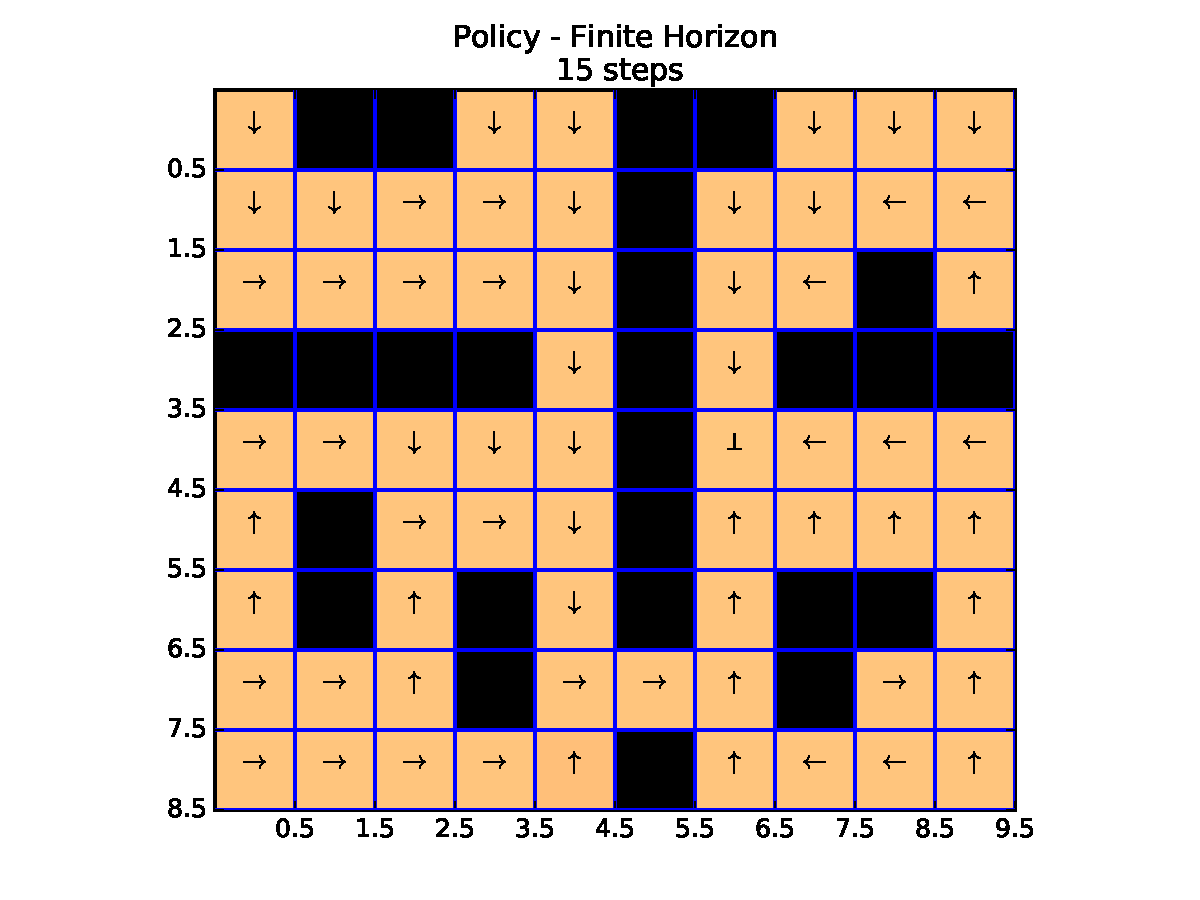
\includegraphics[scale=0.4]{Gridworld/policy_Fin_15.pdf}
	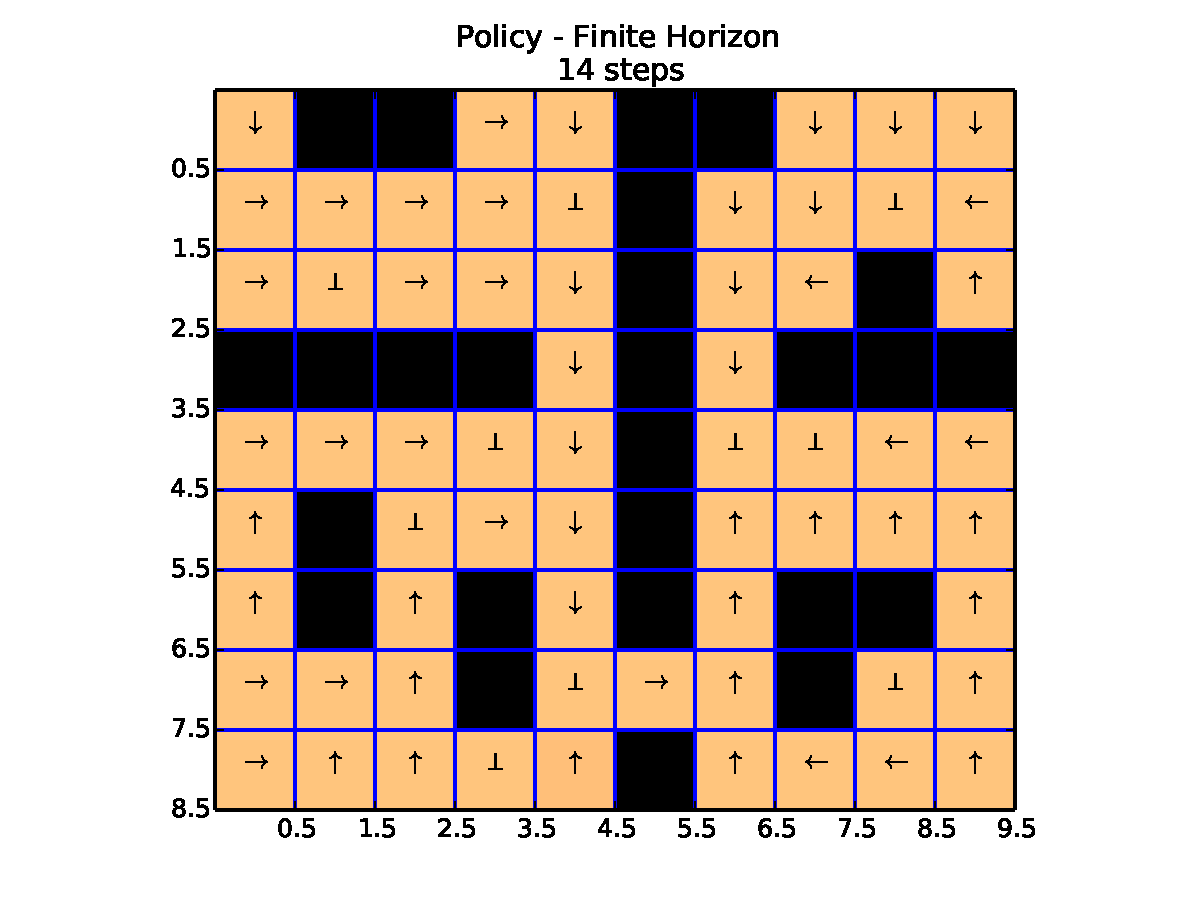
\includegraphics[scale=0.4]{Gridworld/policy_Fin_14.pdf}\\
	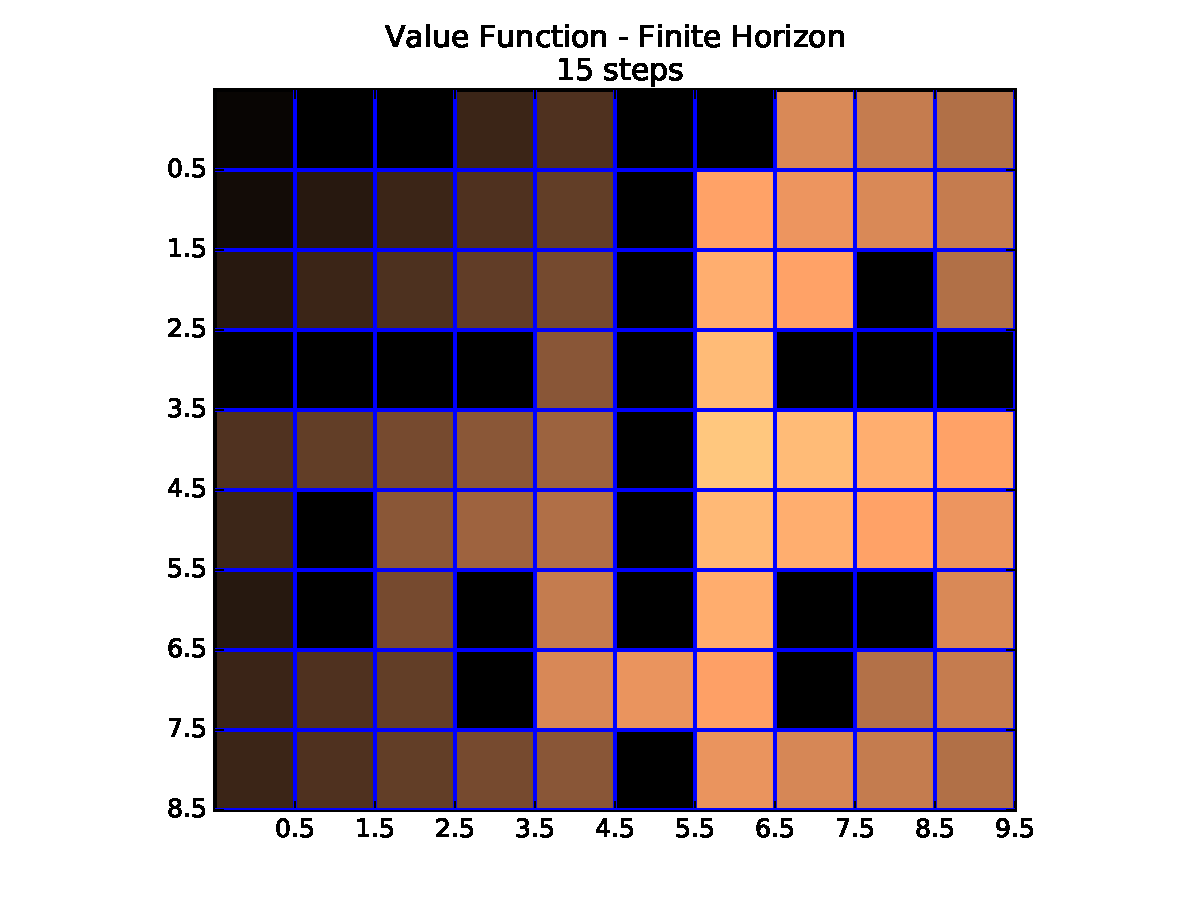
\includegraphics[scale=0.8]{Gridworld/value_Fin_15.pdf} 


	Our policy seems appropriate given our explanation. The robot does collect dirt if it is far enough away from the toy (5,1) but otherwise will prioritize getting towards the toy. It seems so reckless that it even walks over the cat space to get to it when starting in (9,4). This however changes once the robot is limited to 14 steps forcing our robot to simply collect dirt beside the cat in (9,4). 
\end{answer}

\end{question}

%----------------------------------------------


\begin{question}{Infinite Horizon Problem - Part 1}{4}
We now consider the infinite horizon problem, where $T=\infty$. Rewrite Equation~\eqref{Eq:J} for the infinite horizon case adding a discount factor $\gamma$. Explain briefly why the discount factor is needed.

\begin{answer}\end{answer}

\end{question}

%----------------------------------------------


\begin{question}{Infinite Horizon Problem - Part 2}{6}
Calculate the optimal actions with the infinite horizon formulation. Use a discount factor of $\gamma=0.8$ and attach the new policy and value function plots.
What can we say about the new policy? Is it different from the finite horizon scenario? Why?

\begin{answer}\end{answer}

\end{question}

%----------------------------------------------


\begin{question}{Finite Horizon Problem with Probabilistic Transition Function}{10}
After a fight with the cat, the robot experiences control problems. 
For each of the actions \textit{up, left, down, right}, the robot has now a probability $0.7$ of correctly performing it and a probability of $0.1$ of performing another action according to the following rule: if the action is \textit{left} or \textit{right}, the robot could perform \textit{up} or \textit{down}. If the action is \textit{up} or \textit{down}, the robot could perform \textit{left} or \textit{right}.
Additionally, the action can fail causing the robot to remain on the same state with probability $0.1$.
Using the finite horizon formulation, calculate the optimal policy and the value function. Use a time horizon of $T=15$ steps as before. Attach your plots and comment them: what is the most common action and why does the learned policy select it?

\begin{answer}\end{answer}

\end{question}

%----------------------------------------------


\begin{question}[bonus]{Reinforcement Learning - Other Approaches}{8}
What are the two assumptions that let us use the Value Iteration algorithm? What if they would have been not satisfied? Which other algorithm would you have used? Explain it with your own words and write down its fundamental equation.

\begin{answer}
	The Value Iteration algorithm uses the assumptions that we perfectly know our enviroment, that it is a Markov Decision Process process. We can assume that we know our enviroment and we also know it to be computable as it is discrete and finite.
\end{answer}
\end{question}


\end{questions}
